\documentclass[a4paper,12pt]{scrartcl}
\usepackage[utf8x]{inputenc}
\usepackage[T1]{fontenc} % avec T1 comme option  d'encodage c'est ben mieux, surtout pour taper du français.
%\usepackage{lmodern,textcomp} % fortement conseillé pour les pdf. On peut mettre autre chose : kpfonts, fourier,...
\usepackage[french]{babel, varioref} %Sans ça les guillemets, amarchpo
\usepackage{amsmath}
\usepackage{multicol}
\usepackage{amssymb}
\usepackage{tkz-tab}
\usepackage{exercice_sheet}
\flushbottom
\raggedbottom

%\trait
%\section*{}
%\exo{}
%\question{}
%\subquestion{}

\date{}

% Title Page
\title{Exercices de révision, corrigé}

\author{}

\begin{document}

\selectlanguage{french}

\maketitle

%\begin{multicols}{2}
\exo{Suites arithmétiques}

\question{}
La suite est arithmétique de premier terme $u_0 = 5$ et de raison 3. Son terme général est donc $u_n = u_0 + r \times n$.

Le 36ème terme (qui s'appelle $u_{35}$ car on commence à compter à 0) est $u_{35}$. $u_{35} = 5 + 3 \times 35 = 110$

\question{}
On sait que $k_0 = 7$ et $k_{14} = 77$ (données de l'énoncé). La suite $(k_n)$ étant arithmétique, son terme général s'écrit $k_n = k_0 + r \times n$.

On peut donc écrire $k_{14} = k_{0} + r \times 14$ soit:

$7 + 14r = 77$

$\Leftrightarrow r = 5$.

\question{}
Pour ce faire, on peut calculer la raison, de la même façon qu'à la question précédente:

On sait que $p_0 = 35$ et $p_{7} = 112$ (données de l'énoncé). La suite $(p_n)$ étant arithmétique, son terme général s'écrit $p_n = p_0 + r \times n$. 

On peut donc écrire $p_{7} = p_{0} + r \times 7$ soit:

$35 + 7r = 112$

$\Leftrightarrow r = 11$. 

On peut donc écrire les 8 termes de la suite en rajoutant 11 à chaque fois:

\begin{multicols}{4}
$p_0 = 35$

$p_1 = 46$

$p_2 = 57$

$p_3 = 68$

$p_4 = 79$

$p_5 = 90$

$p_6 = 101$

$p_7 = 112$
\end{multicols}

\question{}
Ici, on va directement utiliser la formule permettant de calculer la somme de termes consécutifs d'une suite \textbf{arithmétique}, sans même connaître les termes de la suite (uniquement le premier et le dernier de ceux que l'on souhaite additionner). On rappelle que la somme de termes consécutifs d'une suite $(u_n)$ du rang $p$ au rang $n$ s'écrit:

$$S_n = \sum_{i=0}^{n} u_i = (n+1) \times \dfrac{u_0 + u_n}{2} = (\mbox{nombre de termes}) \times \dfrac{\mbox{premier terme} + \mbox{dernier terme}}{2}$$

On peut donc appliquer directement la formule: $S_n = 20 \times \dfrac{5+57}{2} = 620$.

\question{}
Pour montrer qu'une suite est arithmétique, on calcule $u_{n+1} - u_n$.

Ici, $u_n = -3n + 17$ et $u_{n+1} = -3(n+1) + 17$. On a donc:

$u_{n+1} - u_n = (-3(n+1) + 17)-(-3n + 17) = -3(n+1) + 17 + 3n - 17$

Finalement, $u_{n+1} - u_n = -3$.

La suite est donc arithmétique de raison -3.

Le premier terme est $u_0 = -3\times 0 + 17 = 17$

\exo{Suite géométriques}

\question{}
On connaît le premier terme et la raison de la suite géométrique $(u_n)$. On peut donc écrire $u_n = 2 \times 3^n$. 

D'où $u_7 = 2 \times 3^7 = 4374$ et $u_{17} = 2 \times 3^{17} = 258280326$.

\question{}
On rappelle que la somme des termes d'une suite \textbf{géométrique} s'écrit:

$$S_n = \sum_{i=0}^{n} u_i = u_0 \times \dfrac{1-q^{n+1}}{1-q} = \mbox{premier terme} \times \dfrac{1-q^{\mbox{nombre de termes}}}{1-q}$$.

On peut ici directement appliquer la formule: $S = 100 \times \dfrac{1-1.5^{10}}{1-1.5} \approx 635716$.

\question{Erratum : la raison de la suite est $q=1.5$. Avec cette donnée, vous pouvez faire l'exercice...}

La formule de la somme de termes consécutifs d'une suite géométrique est rappelée question précédente. On l'applique ici, en connaissant la raison $q$ et le premier terme $u_0$. Il restera l'inconnue $n$:

$S = u_0 \times \dfrac{1-q^{n+1}}{1-q}$

soit:

$131875 = 10000 \times \dfrac{1-1.5^{n+1}}{1-1.5}$.

$\Leftrightarrow \dfrac{131875}{10000} = \dfrac{1-1.5^{n+1}}{-0.5} = \dfrac{1.5^{n+1}-1}{0.5}$

$\Leftrightarrow 13.1875 \times 0.5 = 1.5^{n+1}-1 \Leftrightarrow 7.59375 = 1.5^{n+1}$.

Comme d'habitude, lorsqu'on a une écriture de type $a^b$, on réécrit $a$: $1.5 = e^{\ln{1.5}}$. On a donc:

$7.59375 = 1.5^{n+1} \Leftrightarrow 7.59375 = e^{\ln{1.5 \times (n+1)}}$.

On obtient donc: $\ln (7.59375) = \ln(1.5) \times (n+1)$.

$n+1 = \dfrac{\ln 7.59375}{\ln 1.5} = 5$.

On a donc $n+1 = 5$ soit $n = 4$.


On rappelle que lorsqu'on \og retire \fg{} $n$\% à une valeur $x$, cela revient à faire le calcul suivant:

\og $x$ moins $n$\% \fg{} s'écrit $x - x\dfrac{n}{100} = x \left( 1 - \dfrac{n}{100} \right)$. Donc si par exemple on retire 10\%, cela revient bien à multiplier la valeur de départ par 0.9.

\probleme{}

La machine se dépréciant de 20\% d'une année sur l'autre. Cela revient à dire que d'une année sur l'autre, la valeur de la machine est multipliée par 0.8.

\subquestion{}
$V_1 = V_0 \times 0.8 = 7200$

$V_2 = V_1 \times 0.8 = 5760$

\subquestion{}
Pour passer de $V_0$ à $V_1$ puis de $V_1$ à $V_2$, on multiplie par 0.8. Il s'agit donc de 3 termes consécutifs d'une suite géométrique de raison 0.8.

\subquestion{}

$V_3 = 9000 \times 0.8^3 = 4608$

$V_4 = 9000 \times 0.8^4 = 3686.4$

\subquestion{}

La valeur initiale de la machine est de 9000 €. On cherche donc quand la valeur de la machine passe en deçà de 4500 €. Cela revient à résoudre l'inéquation $V_n < 4500$, soit $9000 \times 0.8^n < 4500$

On remarque qu'à la question précédente, le terme $V_4$ est inférieur à 4500. On peut donc répondre que la valeur de la machine devient inférieure à la moitié de sa valeur initiale au bout de 4 ans.

Si on a pas remarqué cela, on peut faire le raisonnement suivant, plus long:

$\Leftrightarrow 0.8^n < \dfrac{1}{2}$

Or, $0.8 = e^{\ln 0.8}$, donc $e^{n \times \ln 0.8} < \dfrac{1}{2}$.

D'où $n \times \ln 0.8 < \ln \left(\dfrac{1}{2}\right)$

Attention, il faut noter que $\ln0.8 < 0$. Donc lorsqu'il va passer de l'autre côté du signe =, l'inégalité changera de sens. Ainsi :

$n > \dfrac{\ln \left(\dfrac{1}{2}\right)}{\ln 0.8}$.

Soit $n > 3.1$, soit au bout de 4 années.

\probleme{Téléobjectif}

Schématisons la situation (figure \vref{objo}):

\begin{figure}
\begin{center}
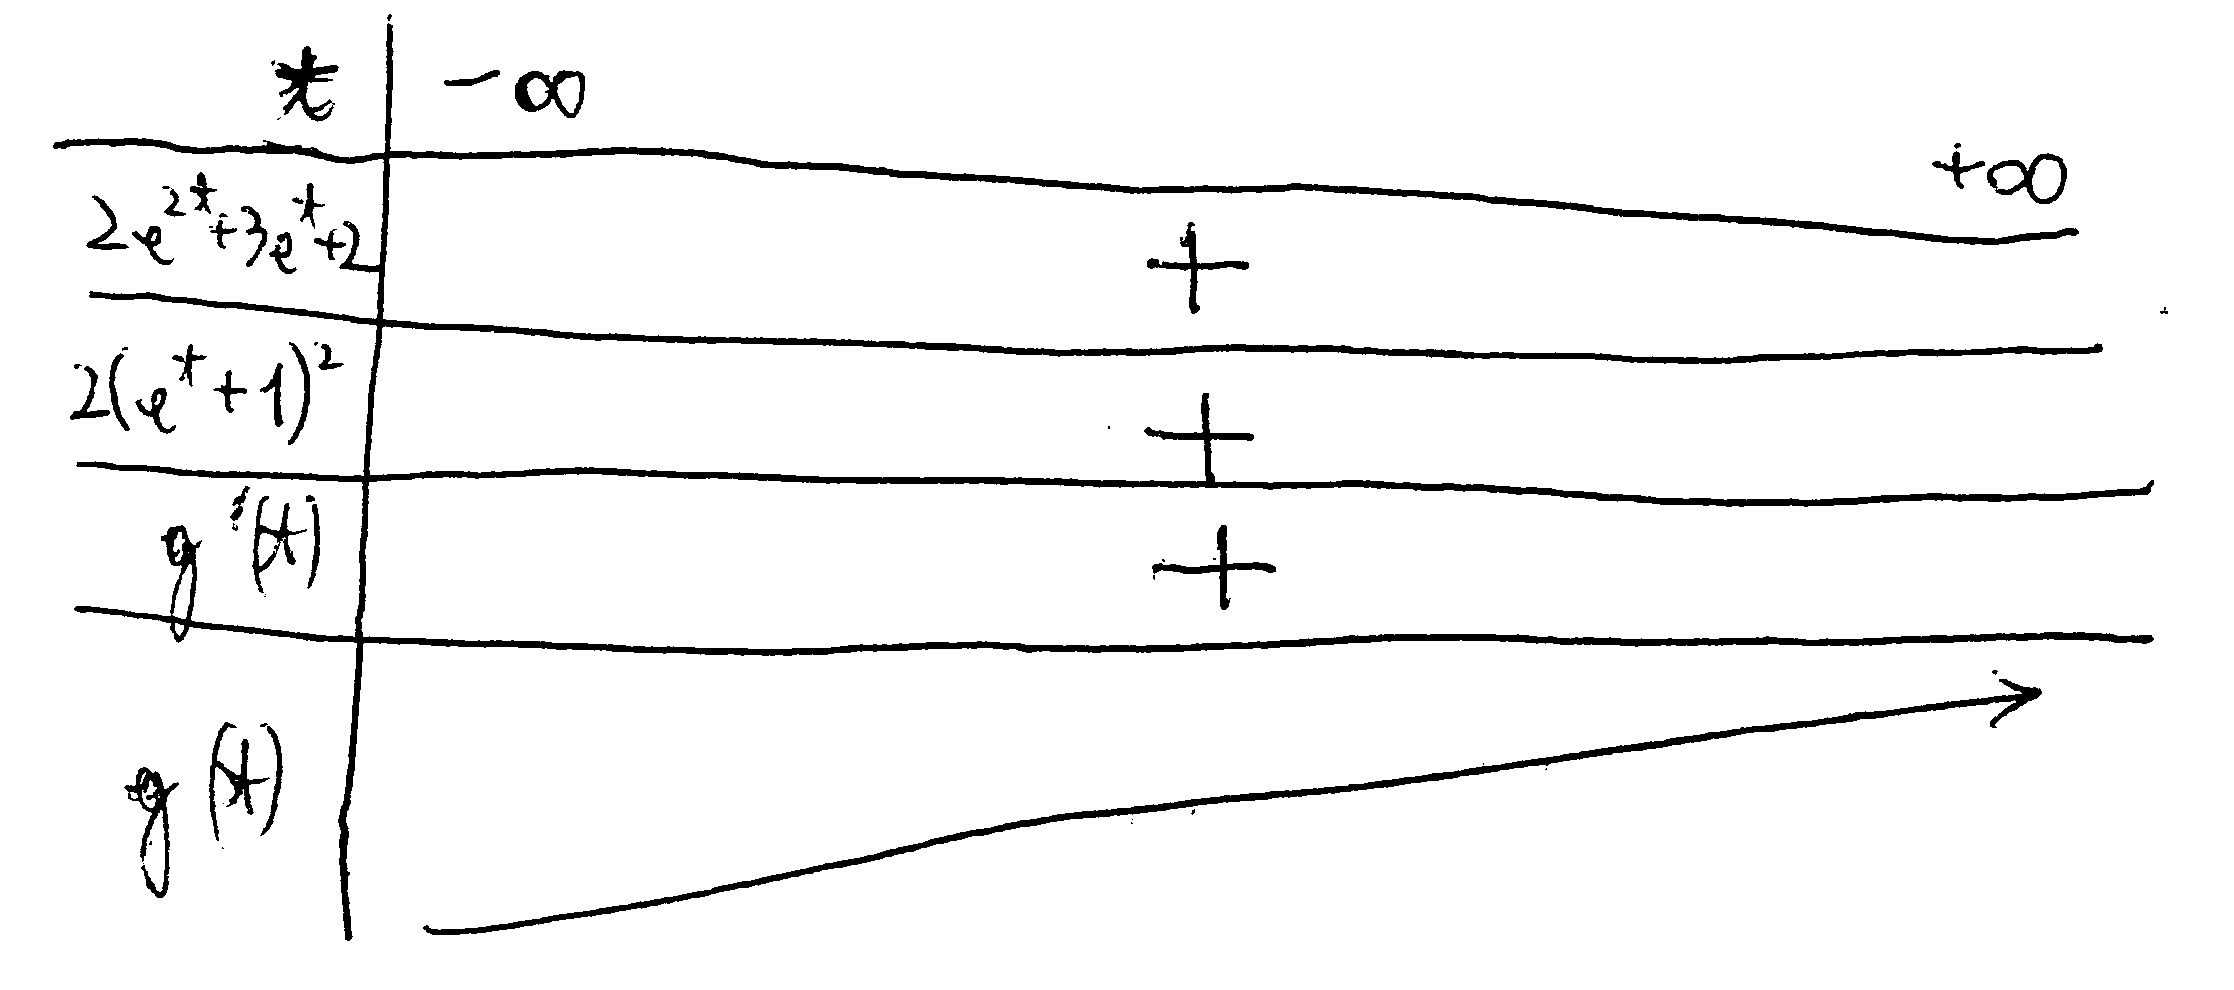
\includegraphics[width=0.7\textwidth]{Pics/1.pdf}
\end{center}
\caption{schéma du téléobjectif}
\label{objo}
\end{figure}

Après le passage d'une lentille, il reste 96\% de la lumière incidente. Ainsi, $I_{n+1} = I_{n} \times 0.96$. Il s'agit bien d'une relation de récurrence. Plus précisément, celle d'une suite géométrique de raison $q = 0.96$. Le premier terme étant $I_0$ qui correspond à l'intensité lumineuse incidente de la première lentille de l'objectif.

Après la 5ème lentille, l'intensité lumineuse restante donc $I_5 = I_0 \times 0.96^5 = I_0 \times 0.81537$.

L'intensité lumineuse frappant la surface sensible (le capteur ou la pellicule) est donc 81.5\% de l'intensité lumineuse incidente $I_0$.

\probleme{}

\partie{}

\question{}

$u_1 = 0.6 u_0 + 200 = 740$

$u_2 = 0.6 u_1 + 200 = 644$

\question{}

\subquestion{}

On veut démontrer que $(v_n)$ est \textbf{géométrique}, on va donc calculer $\dfrac{v_{n+1}}{v_n}$.

Pour ce faire, on va exprimer $v_{n+1}$ en fonction de $v_n$:

D'après l'énoncé, $v_{n+1} = u_{n+1} - 500$. Or, $u_{n+1} = 0.6 u_n + 200$ et $u_n = v_n + 500$ (déduit de ce qu'indique l'énoncé). 

En remplaçant $u_n$ par son expression, on obtient $u_{n+1} = 0.6 \times (v_n + 500) + 200$.

On peut maintenant remplacer $u_{n+1}$ par son expression et obtenir $v_{n+1}$ en fonction de $v_n$:

$$v_{n+1} = (0.6 \times (v_n + 500) + 200) - 500$$

Soit $v_{n+1} = 0.6 v_n$. La raison de la suite est 0.6.

Le premier terme: $v_0 = u_0 - 500 = 400$. 

\subquestion{}
On déduit de ce qui précède (elle est géométrique, on connaît sa raison et son premier terme):

$v_n = 400 \times 0.6^n$.

\subquestion{}
$u_n = v_n+500$, d'où $u_n = 400 \times 0.6^n+500$

\subquestion{OL uniquement}

$(v_n)$ est géométrique de raison $q=0.6$. Donc $|q|<1$. Donc $\lim\limits_{n\to\infty} v_n = 0$ (cf. cours).

Or, $u_n = v_n + 500$, d'où $\lim\limits_{n\to\infty} u_n = 500$.

\partie{}

\question{}

\subquestion{}
En 2006, la société A a 900 clients dans l'échantillon, la société B en possède 100.

\littlestar{En 2007}

\begin{itemize}
\item La société A cède 20\% de sa clientèle soit 180 clients.
\item La société A récupère 20\% de la clientèle de B, soit 20 clients.
\end{itemize}

Elle a donc au total perdu 160 clients. $900 - 160 = 740$.

\littlestar{En 2008}

\begin{itemize}
\item La société A cède 20\% de sa clientèle soit 148 clients.
\item La société A récupère 20\% de la clientèle de B, soit 52 clients.
\end{itemize}

Elle a donc au total perdu 96 clients. $740 - 96 = 644$.

\subquestion{}
La suite $(a_n)$:

La clientèle de l'entreprise B est $1000-a_n$ (le total moins les clients de l'entreprise A). L'entreprise A récupère 20\% de cette clientèle, soit $0.2 \times (1000-a_n)$.

Mais elle perd 20\% de sa propre clientèle. Ainsi, il lui en reste 80\% l'année d'après: $0.8 a_n$. 

À l'année $n+1$, sa clientèle est donc $a_{n+1} = 0.8 a_n + 0.2 \times (1000-a_n)$ qui se développe et réduit en $a_{n+1} = 0.6 a_n + 200$.

\question{}
La suite $(a_n)$ est égale à la suite $(u_n)$ de la partie 1. Sa limite est donc 500. La tendance est donc que les 2 entreprises vont se partager la moitié du marché des télécoms dans la pays (500 chacune).

\probleme{Employés}

\question{Terme général}

\subquestion{}

$u_0 = 1500$

$u_1 = 1450$

$u_2 = 1405$

Si $(u_n)$ était arithmétique, on rajouterait chaque année un nombre constant d'employés. Ce n'est pas le cas.

Si $(u_n)$ était géométrique, on multiplierait chaque année le nombre d'employés par un même nombre. Ce n'est pas le cas non plus.

$(u_n)$ n'est donc ni géométrique ni arithmétique.

\subquestion{}

\og{}Retirer\fg{} 10\% revient à multiplier la valeur de l'année précédente par 0.9. Embaucher 100 nouvelles personnes revient à additionner 100. On a donc $u_{n+1} = 0.9 u_n + 100$.

\question{}
Suite $v_n$

\subquestion{}

D'après l'énoncé, $v_{n} = u_{n} - 1000$. Donc $v_{n+1} = u_{n+1} - 1000$\footnote{Si quelque-chose est vrai au rang $n$, ça l'est aussi au rang $n+1$.}.

Or, $u_{n+1} = 0.9u_n + 100$ (question précédente) donc $v_{n+1} = 0.9u_n + 100 - 1000 = 0.9u_n - 900$. 

Mais, on peut déduire de l'énoncé que $u_n = v_n + 1000$. Donc : $v_{n+1} =  0.9 \cdot (v_n + 1000) - 900 = 0.9 v_n$ 

\subquestion{}
La suite $v_n$ est définie par récurrence comme démontré précédemment: $v_{n+1} = 0.9 v_n$. Il s'agit donc d'une suite géométrique de raison $q = 0.9$ et de premier terme $v_0 = u_0 - 1000 = 500$.

On peut donc écrire (par définition) que $v_n = 500 \times 0.9^n$.

Comme on l'a déduit plus haut, $u_{n} = v_{n} + 1000$, donc $u_{n} = 500 \times 0.9^n + 1000$

\subquestion{OL uniquement}
$(v_n)$ est une suite géométrique de raison $q = 0.9$, donc $|q| < 1$, on peut donc en déduire que $\lim\limits_{n\to\infty} u_n = 1000$.

\question{}
Il s'agit de la même situation, sauf qu'ici $u_0 = 1500+300 = 1800$. On a donc ici:

$u_0 = 1800$

$u_1 = 1720$

$u_2 = 1648$

$u_3 = 1583$

$u_4 = 1525$

$u_5 = 1472$

L'année à partir de laquelle l'entreprise ne sera plus en sur-effectif correspond au rang 5 de na suite ($n = 5$), ce qui correspond à l'année $2006 + 5$, soit l'année 2011.

\probleme{Forage}

\partie{Calcul de coûts}

\question{}
Il suffit d'ajouter 20€ au coût du 3\textsuperscript{ème} mètre $240+20 = 260$.

\question{}
$200+220+240+260 = 920$. Le coût est donc de 920€.

\partie{Étude d'une suite}

\question{}
Pour passer d'un terme au suivant, on rajoute 20. La suite est donc arithmétique, de raison 20.

\question{}
Le premier terme $u_0$ est 200. On peut donc écrire $u_n = 200 + 20 n$.

\question{}
D'après la question précédente: $u_{10} = 200 + 20 \times 10 =400$.

\partie{Exploitation}

\question{}
Pour calculer le coût total d'un forage de 11 mètres de profondeur, il nous faut calculer la somme des termes de $u_0$ à $u_{10}$:

$C_{10} = \sum\limits_{i=0}^{10} u_i$ soit:

$C_{10} = (n+1) \times \dfrac{u_0+u_{10}}{2}$ où $n+1$ est le nombre de termes additionnés.

On a donc $C_{10} = 11 \times \dfrac{200+400}{2} = 3300$. 

Le coût total d'un forage de 11m est donc de 3300€.

\question{}
De la même manière que précédemment, on va exprimer la somme $C_n$:

$C_n = n \times \dfrac{u_0+u_{n-1}}{2}$. Or, $u_{n-1} = 200 +20(n-1)$ et $u_0 = 200$. D'où:

$$C_n = n \times \dfrac{200 + 200 + 20(n-1)}{2} = n \times (200 + 10(n-1))$$

$$C_n = n \times (200 + 10(n-1)) = n \times (190 + 10n) = 190n + 10n^2$$

\question{}
Il s'agit de résoudre l'inéquation $C_n \leqslant 6500$.

Soit: $10n^2 + 190n - 6500 \leqslant 0 \Leftrightarrow n^2 + 19n - 650 \leqslant 0$.

Il s'agit d'un polynôme du second degré. 

$\Delta = 19^2 + 4 \times 650 = 2961 = 3 \sqrt{329}$.

Le polynôme a donc 2 racines.

Rappel: $n_{1,2} = \dfrac{-b \pm \sqrt{\Delta}}{2a}$

$$n_1 = \dfrac{-190 - 3 \sqrt{329}}{2} \approx -36.7$$

$$n_2 = \dfrac{-190 + 3 \sqrt{329}}{2} \approx 17.7$$

Ce polynôme a un $a$ positif et est donc négatif sur $[n_1;n_2]$.

L'inéquation est donc vérifiée pour $n_1 \leqslant n \leqslant n_2$. Or, la profondeur du forage est forcément un nombre positif, donc $n \leqslant n_2$. Comme $n$ est un nombre entier, $0 \leqslant n \leqslant 17$.

Avec un budget de 6500€, on peut donc atteindre une profondeur de 17m.

\probleme{Nouvel atelier}

\question{}
Pour montrer que la production est croissante, il suffit de montrer que $u_{n+1} \geqslant u_n$:

%$u_{n+1} = 80 - 27 e^{-0.1(n+1)}$

%$u_{n+1} = 80 - 27 e^{-0.1n - 0.1}$

%$u_{n+1} = 80 - 27 e^{-0.1n} \times e^{- 0.1}$

$-0.1 < 0$ d'où $e^{-0.1} < e^0$ soit $0 < e^{-0.1} < 1$ (la fonction exponentielle étant croissante et strictement positive).

On peut donc poursuivre: 

$e^{-0.1} < 1$

$\Leftrightarrow 27 e^{-0.1n}e^{-0.1} < 27 e^{-0.1n}$ car $27 e^{-0.1n} > 0$

$\Leftrightarrow  -27 e^{-0.1n}e^{-0.1} > -27 e^{-0.1n}$

$\Leftrightarrow 80-27 e^{-0.1n}e^{-0.1} > 80-27 e^{-0.1n}$

$\Leftrightarrow u_{n+1} \geqslant u_n$.

Cela signifie que pour tout entier naturel $n$, le terme de rang $n+1$ est plus grand que le terme de rang $n$. La suite est donc croissante.

\question{}
On cherche $n$ tel que $u_n > 72$.

Soit : $80-27 e^{-0.1n} \geqslant 72$. 

$\Leftrightarrow 8 \geqslant 27 e^{-0.1n}$

$\Leftrightarrow \dfrac{8}{27} \geqslant e^{-0.1n}$

$\Leftrightarrow \ln \left( \dfrac{8}{27} \right) \geqslant -0.1n$

$\Leftrightarrow -10 \times \ln \left( \dfrac{8}{27} \right) \leqslant n$

$\Leftrightarrow -10 \times \ln \left( \dfrac{8}{27} \right) \approx 12.6$

La production dépasse donc les 72 unités au 13\textsuperscript{ème} jour.

\question{Suite $v_n$.}

\subquestion{}
Pour ce faire, comme à chaque fois on calcule le quotient $\dfrac{v_{n+1}}{v_n}$.

$\dfrac{v_{n+1}}{v_n} = \dfrac{e^{-0.1(n+1)}}{e^{-0.1n}} = \dfrac{e^{-0.1n - 0.1}}{e^{-0.1n}}$

Donc $\dfrac{v_{n+1}}{v_n} = \dfrac{e^{-0.1n} \times e^{-0.1}}{e^{-0.1n}} = e^{-0.1}$ (par simplification).

La suite $(v_n)$ est donc géométrique de raison $e^{-0.1}$.

\subquestion{}
$S = \sum\limits_{i = 1}^{12} = v_1 \times \dfrac{1-q^{n}}{1-q}$

On a donc $S = e^{-0.1} \times \dfrac{1-e^{-0.1\times 12}}{1-e^{-0.1}} \approx 6.64$.

\question{}
D'après la question précédente, 6 unités auront été produites durant les 12 premiers jours.




\end{document}
